\subsection{Примеры неустойчивых стационарных решений}

\newtheorem{exmp_bur}{Пример}
\begin{exmp_bur}
\end{exmp_bur}

Начальное условие $\theta_0(x) = \frac{\sin(\pi x)}{G(x)}$, параметр $\sigma$ возмем равный 3. Из предыдущего параграфа известно, что система устойчива для данного параметра. На рисунке 1 представлено численное решение без управления, рисунке 2 управление включено.

\begin{figure}[H]
\centering
\begin{minipage}{.5\textwidth}
  \centering
  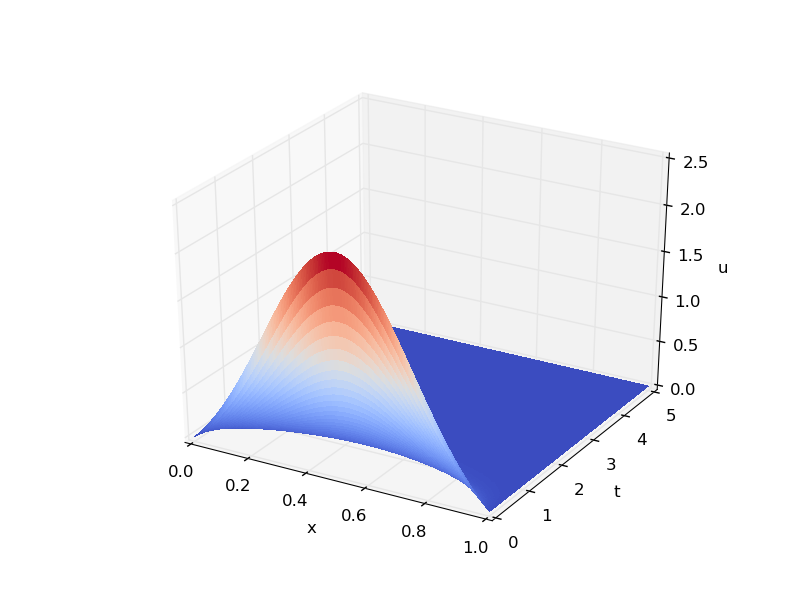
\includegraphics[width=3.5in]{ex_s3}
  \caption{Без управления}
  \label{fig:test1}
\end{minipage}%
\begin{minipage}{.5\textwidth}
  \centering
  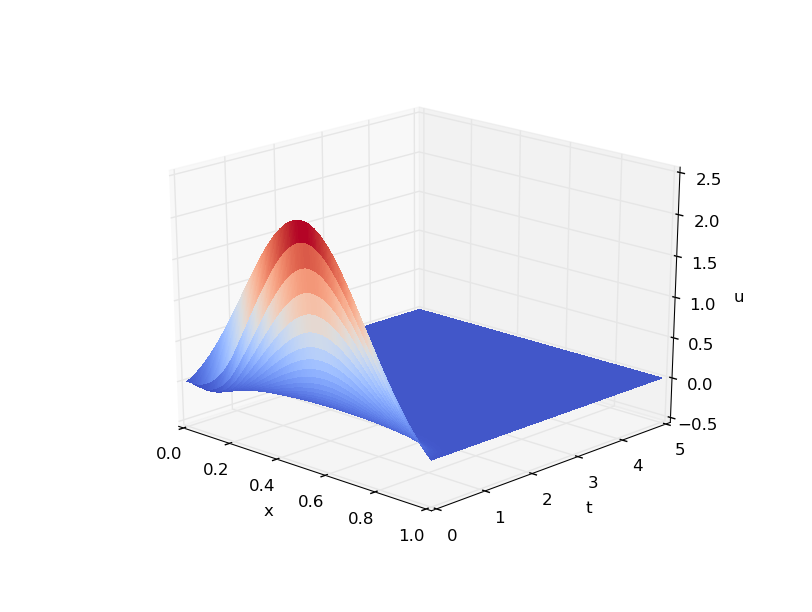
\includegraphics[width=3.5in]{re_s3}
  \caption{Управление с $m = 2, \; r = 15$}
  \label{fig:test2}
\end{minipage}
\end{figure}


\begin{exmp_bur}
\end{exmp_bur}
Начальное условие то же самое, что и в предыдущем примере. Параметр $\sigma$ возмем равный 15. На рисунке 3 показано неустойчивое поведение системы без управления, а сама стабилизация с параметрами $\omega = [0, 0.2], \; r = 15, \; m = 2$ предоставлена на рисунке 4.


\begin{figure}[H]
\centering
\begin{minipage}{.5\textwidth}
  \centering
  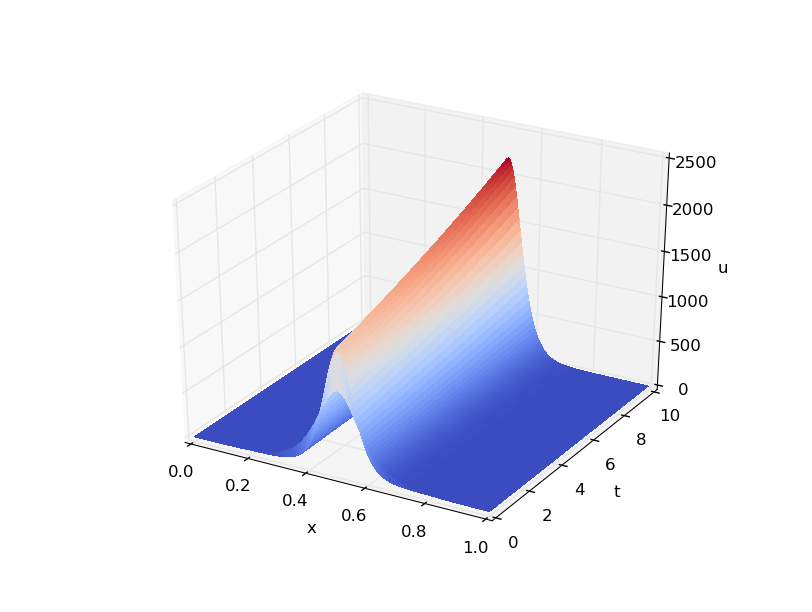
\includegraphics[width=3.5in]{ex_s15}
  \caption{Без управления}
  \label{fig:test1}
\end{minipage}%
\begin{minipage}{.5\textwidth}
  \centering
  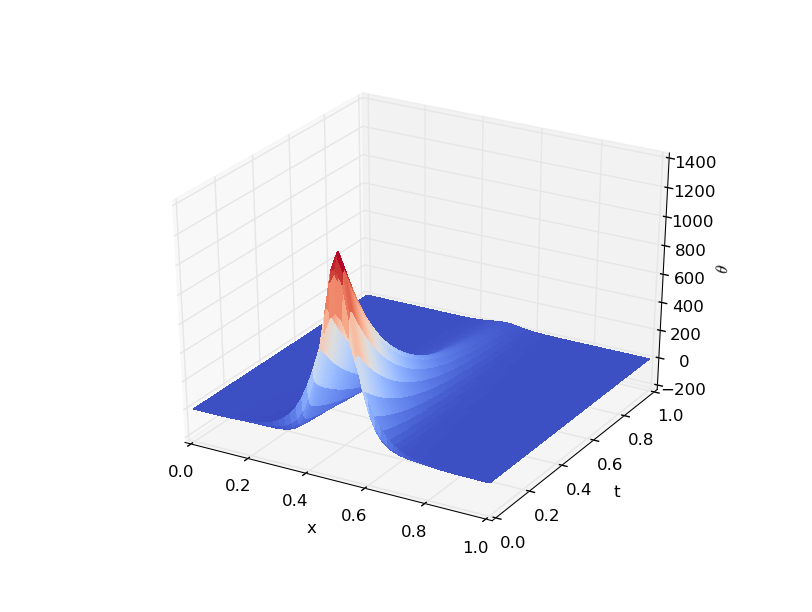
\includegraphics[width=3.5in]{re_s15}
  \caption{Управление с $m = 2, \; r = 15$}
  \label{fig:test2}
\end{minipage}
\end{figure}


\begin{exmp_bur}
\end{exmp_bur}
В качестве начального условия возмем быстро осциллирующую функцию $\frac{\sin(10 \pi x)}{G(x)}$. Параметр $\sigma$ возмем равным 15. На рисунке 5 поведение системы без управления, рисунок 6 - управление с $\omega = [0, 0.2], \; r = 15, \; m = 2$.

\begin{figure}[H]
\centering
\begin{minipage}{.5\textwidth}
  \centering
  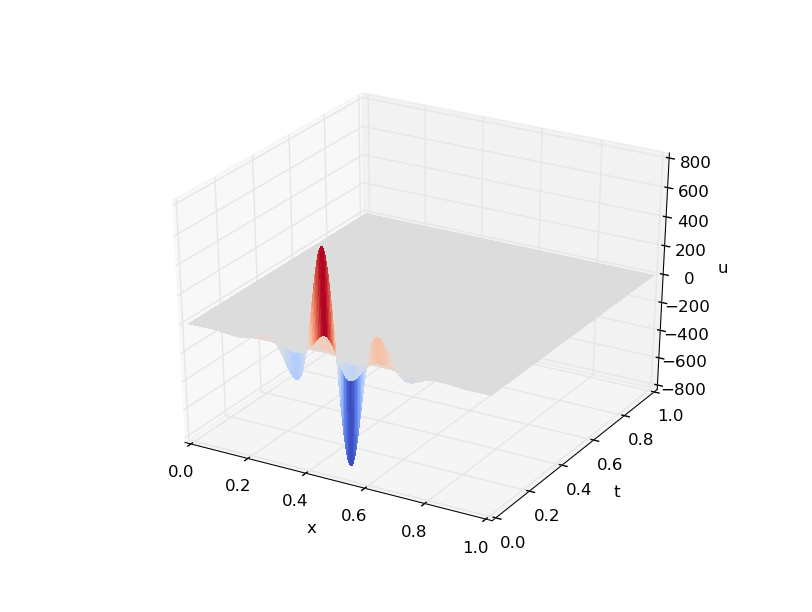
\includegraphics[width=3.5in]{ex_sin10_s15}
  \caption{Без управления}
  \label{fig:test1}
\end{minipage}%
\begin{minipage}{.5\textwidth}
  \centering
  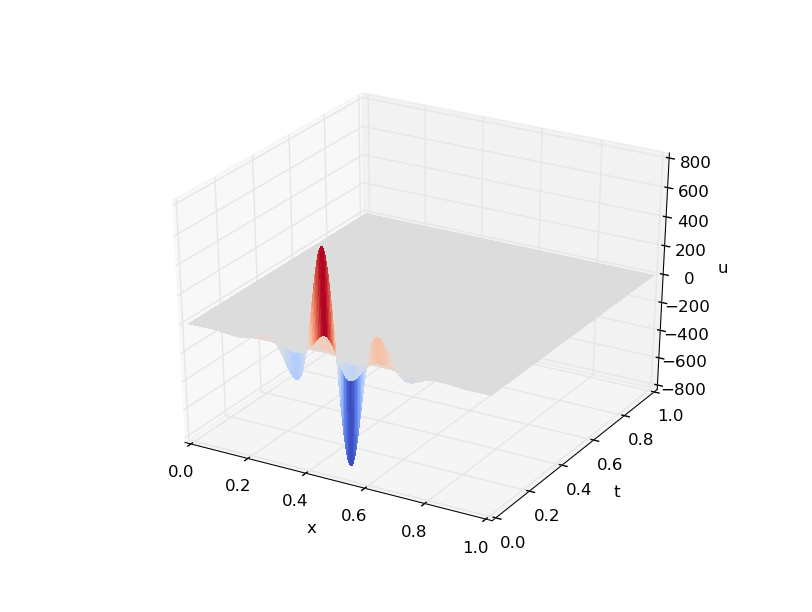
\includegraphics[width=3.5in]{re_sin10_s15}
  \caption{Управление с $m = 2, \; r = 15$}
  \label{fig:test2}
\end{minipage}
\end{figure}


\begin{exmp_bur}
\end{exmp_bur}
Теперь начальное условия $\theta_0(x) = \frac{x^2}{G(x)}$. Фиксируем $\omega = [0, 0.2]$, $\sigma = 15$. 

\begin{figure}[H]
\centering
\begin{minipage}{.5\textwidth}
  \centering
  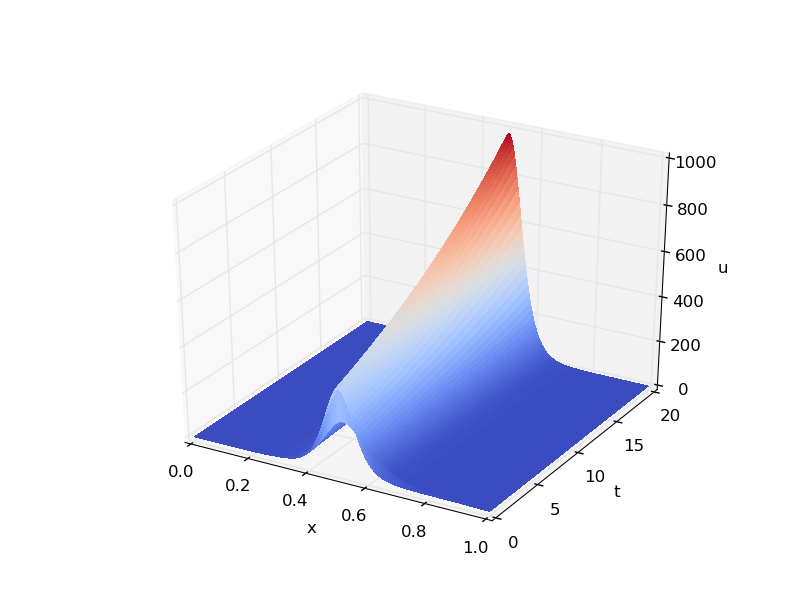
\includegraphics[width=3.5in]{ex_x2_s15}
  \caption{Без управления}
  \label{fig:test1}
\end{minipage}%
\begin{minipage}{.5\textwidth}
  \centering
  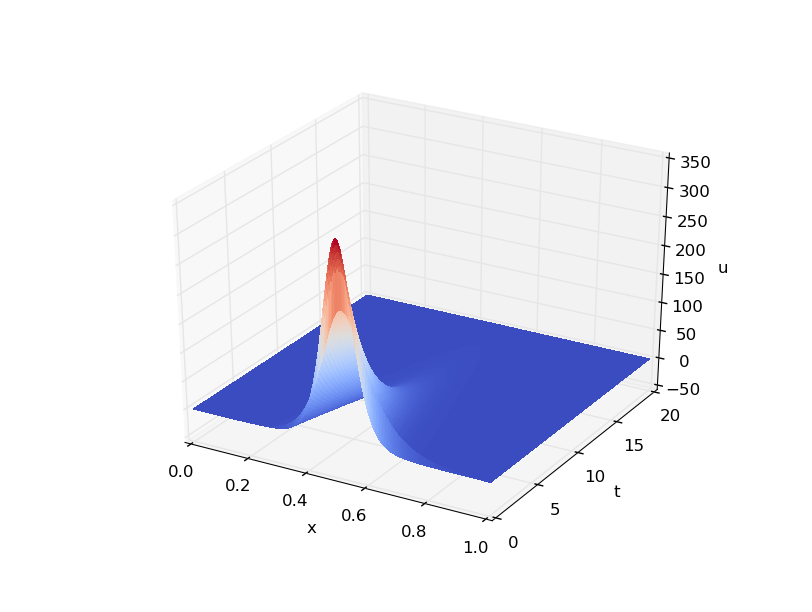
\includegraphics[width=3.5in]{re_x2_s15}
  \caption{$\omega = [0, 0.2], \; r = 15, \; m = 2$}
  \label{fig:test2}
\end{minipage}
\end{figure}

